%%%%%%%%%%%%%%%%%%%%%%%%%%%%%%%%%%%%%%%%%%%%%%%%%%%%%%%%%%%%%%%%%%%%%%%%%%%%%%%%
% INTRODUCTION
\chapter{Introduction}
%%%%%%%%%%%%%%%%%%%%%%%%%%%%%%%%%%%%%%%%%%%%%%%%%%%%%%%%%%%%%%%%%%%%%%%%%%%%%%%%

File system metadata management for a global namespace is difficult to scale.
The attention that the topic has received, in both industry and academia,
suggests that even decoupling metadata IO from data IO so that these services
can scale independently~\cite{alam:pdsw2011-metadata-scaling,
ghemawat:sosp2003-gfs, hildebrand:msst2005-pnfs, weil:osdi2006-ceph,
welch:fast08-panasas, xing:sc2009-skyfs} is insufficient for today's
workloads. In the last 20 years, many cutting-edge techniques for scaling file
system metadata access in a single namespace have been proposed; most
techniques target POSIX IO's global and hierarchical semantics.

Unfortunately, techniques for scaling file system metadata access in a global
namespace are implemented in `clean-slate' file systems built from the ground
up. To leverage techniques from different file systems, administrators must
provision separate storage clusters, which complicates management because
administrators must now (1) configure data migrations across file system
boundaries and (2) compare techniques by understanding internals and
benchmarking systems.  Alternatively, developers that want the convenience of a
single global namespace can integrate multiple techniques into an existing file
system and expose configuration parameters to let users select metadata
management strategies.  While this minimizes data movement and lets users
compare techniques, it makes a single system more difficult to understand and
places the burden on file system developers to modify code every time a new
technique is needed or becomes available.

As a result of this complexity and perceived scalability limitation,
communities are abandoning global namespaces. But using different storage
architectures, like object stores, means that legacy applications must be
re-written and users must be re-trained to use new APIs and services. We make
global namespaces scalable with the fundamental insight that many file systems
have similar internals and that the policies from cutting-edge techniques for
file system metadata management can be expressed in a system-agnostic way.

Driven by this insight, we make global namespaces scalable by designing
domain-specific policies that guide internal file system metadata management
techniques. We build a programmable file system with APIs that let developers
of higher-level software ({\it i.e.} layers above the file system) express
domain-specific knowledge in a storage-agnostic way.  Policy engines embedded
in file system metadata management modules use this knowledge to guide internal
mechanisms. Using these frameworks, we explore the design space of file system
metadata management techniques and design scalable policies for (1) subtree
load balancing, (2) relaxing subtree consistency and durability semantics, and
(3) subtree schemas and generators.  These new, domain-specific customizations
make metadata management more scalable and, thanks to our frameworks, these
policies can be compared to approaches from related work. 

\section{Contributions}

The first contribution is an API and policy engine for file system metadata,
where administrators inject custom subtree load balancing logic that controls
``when" subtrees are moved, ``where" subtrees are moved, and ``how much"
metadata to move at each iteration.  We design and quantify load balancing
policies that constantly adapt, which work well for mixed workloads ({\it
e.g.}, compiling source code), policies that aggressively shed half their load,
which work well for create-heavy workloads localized to a directory, and
policies that shed parts of their load when a server's processing capacity is
reached, which work well for create-heavy workloads in separate directories.
We also show how the data management language and policy engine designed
for file system metadata turns out to be an effective control plane for general
load balancing and cache management.

The second contribution is an API and policy engine that lets administrators
specify their consistency/durability requirements and dynamically assign them
to subtrees in the same namespace; this allows administrators to optimize
subtrees over time and space for different workloads. Letting different
semantics co-exist in a global namespaces scales further and performs better
than systems that use one strategy.  Using our framework we custom-fit subtrees
to use cases and quantify the following performance improvements:
checkpoint-restart jobs are almost an order of magnitude faster when fully
relaxing consistency, user home directory workloads are close to optimal if
interference is blocked, and the overhead of checking for partial results is
negligible given the optimal heartbeat interval.

The third contribution is a methodology for generating namespaces automatically
and lazily, without incurring the costs of traditional metadata management,
transfer, and materialization.  We introduce namespace generators and schemas
to describe file system metadata structure in a compact way. If clients and
servers can express the namespace in this way, they can compact metadata,
modify large namespaces more quickly, and generate only relevant parts of the
namespace. The result is less network traffic, storage footprints, and overall
metadata operations.  

In addition to academic publications, these contributions and their
corresponding prototypes have received considerable attention in the community.
Mantle was merged into Ceph and funded by the Center for Research in Open
Source Software and Los Alamos National Laboratory; Malacology and Mantle were
featured in the Next Platform magazine and the 2017 Lua Workshop; and our
papers are some of the first Popper-compliant~\cite{jimenez:login16-popper,
jimenez:ipdpsw17-popper, jimenez_tackling_2015, jimenez_aver_2016,
jimenez:rr18-popper} conference papers\footnote{http://falsifiable.us/}.

\section{Outline}

\begin{figure}[tb]
  \centering
  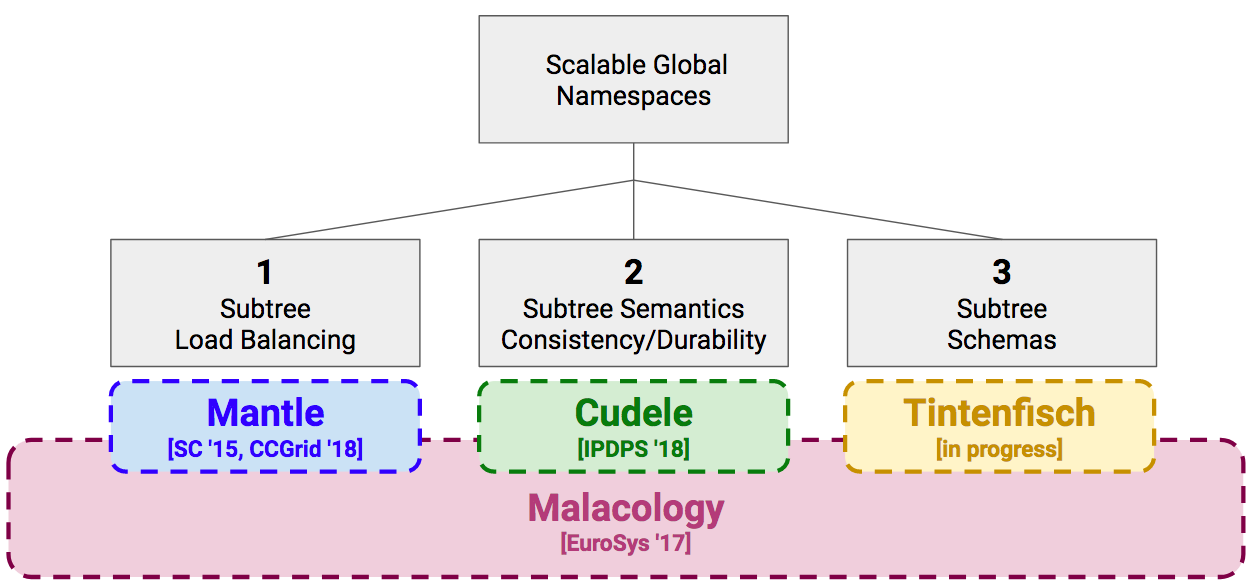
\includegraphics[width=1\textwidth]{./chapters/overview.png}
  \caption{An outline of this thesis.}
  \label{fig:thesis-overview}
\end{figure}

An outline of the thesis is shown in Figure~\ref{fig:thesis-overview}.

Chapter~\ref{chp:related-work} discusses the file system metadata management
problem and shows why today's jobs incur these types of workloads. We also
survey related work for providing scalability while enforcing POSIX IO
semantics. Chapter~\ref{chp:prototyping-platform} describes our prototyping
platform, Ceph, and the interfaces we added to create a programmable storage
system called Malacology. A version of this work appears in EuroSys
2017~\cite{sevilla:eurosys17-malacology}.

Chapter~\ref{chp:mantle} describes the API and policy engine for load balancing
subtrees across a metadata cluster. We motivate the framework by measuring the
advantages of file system workload locality and examining the current CephFS
implementation designed in~\cite{weil:osdi2006-ceph, weil:sc2004-dyn-metadata}.
Our prototype implementation, Mantle, is used for the evaluation. A version of
this work appears in Supercomputing 2015~\cite{sevilla:sc15-mantle}.
Chapter~\ref{chp:mantle-beyond} shows the generality of the approach by using
the API for load balancing in ZLog, an implementation of the
CORFU~\cite{balakrishnan_corfu_2012} API on Ceph, and for cache management in
ParSplice~\cite{perez:jctc20150parsplice}, a molecular dynamics simulation
developed at Los Alamos National Laboratory. A version of this work appears in
CCGrid 2018~\cite{sevilla:ccgrid18-parsplice}.

Chapter~\ref{chp:cudele} describes the API and policy engine for relaxing
consistency and durability semantics in a global file system namespace. We
focus on building blocks called mechanisms and show how administrators can
build application-specific semantics for subtrees.  We motivate the work by
measuring the POSIX IO overheads in CephFS and by examining current workloads
in HPC and in the cloud. Microbenchmarks of our prototype implementation,
Cudele, show the performance of individual mechanisms while the macrobenchmarks
model real-world use cases. A version of this work appears in IPDPS
2018~\cite{sevilla:ipdps18-cudele}.

Even if clients relax consistency and durability semantics in a global
namespace, there are still scenarios where clients create large amounts of file
system metadata that must be transferred, managed, and materialized at read
time; this is another scalability bottleneck for file system metadata access.
Chapter~\ref{chp:tintenfisch} describes our implementation called Tintenfisch,
which lets clients and servers generate subtrees to reduce network traffic,
storage footprints, and file system metadata load. We examine three motivating
examples from three different domains: high performance computing, high energy
physics, and large scale simulations. We then present namespace schemas for
categorizing file system metadata structure and namespace generators for
compacting metadata. A version of this work appears in HotStorage
2018~\cite{sevilla:hotstorage18-tintenfisch}.

Chapter~\ref{chp:conclusion} concludes and outlines future work.

